\documentclass[journal]{vgtc}       % preprint (journal style)

%% Uncomment one of the lines above depending on where your paper is
%% in the conference process. ``review'' and ``widereview'' are for review
%% submission, ``preprint'' is for pre-publication, and the final version
%% doesn't use a specific qualifier. Further, ``electronic'' includes
%% hyperreferences for more convenient online viewing.

%% Please use one of the ``review'' options in combination with the
%% assigned online id (see below) ONLY if your paper uses a double blind
%% review process. Some conferences, like IEEE Vis and InfoVis, have NOT
%% in the past.

%% Please note that the use of figures other than the optional teaser is not permitted on the first page
%% of the journal version.  Figures should begin on the second page and be
%% in CMYK or Grey scale format, otherwise, colour shifting may occur
%% during the printing process.  Papers submitted with figures other than the optional teaser on the
%% first page will be refused.

\usepackage{mathptmx}
\usepackage{graphicx}
\usepackage{times}
\usepackage{caption}
\usepackage{color}
\usepackage{bm}
\usepackage{amsmath}
\usepackage{microtype}
\usepackage[normalem]{ulem}

% options for TODO: either use red bold font for litle annotations (which do not work very well)

\newcommand{\todo}[1]{\textcolor{red}{\textbf{TODO:} #1}}

% following commands are 'non standard' and not bundled with template, delete it problems occur
\usepackage{xargs}                      % Use more than one optional parameter in a new commands
\usepackage[pdftex,dvipsnames]{xcolor}  % Coloured text etc.
%\usepackage[colorinlistoftodos,prependcaption,textsize=tiny]{todonotes}
%\newcommand{\unsure}[1]{\todo[linecolor=red,backgroundcolor=red!25,bordercolor=red,inline]{#1}}
%\newcommand{\change}[1]{\todo[linecolor=blue,backgroundcolor=blue!25,bordercolor=blue,inline]{#1}}
%\newcommand{\info}[1]{\todo[linecolor=OliveGreen,backgroundcolor=OliveGreen!25,bordercolor=OliveGreen,inline]{#1}}
%\newcommand{\improvement}[1]{\todo[linecolor=Plum,backgroundcolor=Plum!25,bordercolor=Plum,inline]{#1}}
%\newcommand{\thiswillnotshow}[1]{\todo[disable,inline]{#1}}



\captionsetup[table]{justification=justified,singlelinecheck=false}
\captionsetup[figure]{justification=justified,singlelinecheck=false}

\vgtcinsertpkg



\title{Comvi - Comparative Visualization of Molecular Surfaces using Similarity-based Clustering}

\author{Wilhelm Buchm\"uller, Shoma Kaiser, Damir Ravilija, Enis ...}
\authorfooter{
\begin{tabular}{cc}
 Wilhelm Buchmüller  & Shoma Kaiser \\
 buch.willi@googlemail.com     & example@example.com \\
 Enis .. . & Damir Rwilja   \\
 example@example.com & example@example.com

\end{tabular}
}



%other entries to be set up for journal
%\shortauthortitle{Schmid \MakeLowercase{\textit{et\,al.}}: ProjINF for fun and profit}


\abstract{
The goal of this paper is to show the reader the abstract methods and concrete applications that were used to extract and compare features  and rank the similarity of the molecular protein maps. Further we present a new method of how the won data can be visualized on high resolution and large displays with a  The paper describes the process and the approaches that were taken to solve this task. 
} 


\keywords{Clustering, Similarity, feature extraction, Visualization, high-resolution display, Powerwall,MegaMol, VISUS}

%% ACM Computing Classification System (CCS).
%% See <http://www.acm.org/class/1998/> for details.
%% The ``\CCScat'' command takes four arguments.

\CCScatlist{ % not used in journal version
	\CCScat{Computer Graphics}{I.3.8}{Applications}{Molecular Dynamics Visualization}
	\CCScat{Simulation and Modeling}{I.6.6}{Simulation Output Analysis}{Molecular Dynamics Visualization}
	\CCScat{Computer Graphics}{I.3.7}{Three-Dimensional Graphics and Realism}{Raytracing}
}

\graphicspath{{pics/}}

% Uncomment below to include a teaser figure.
\teaser{
\centering
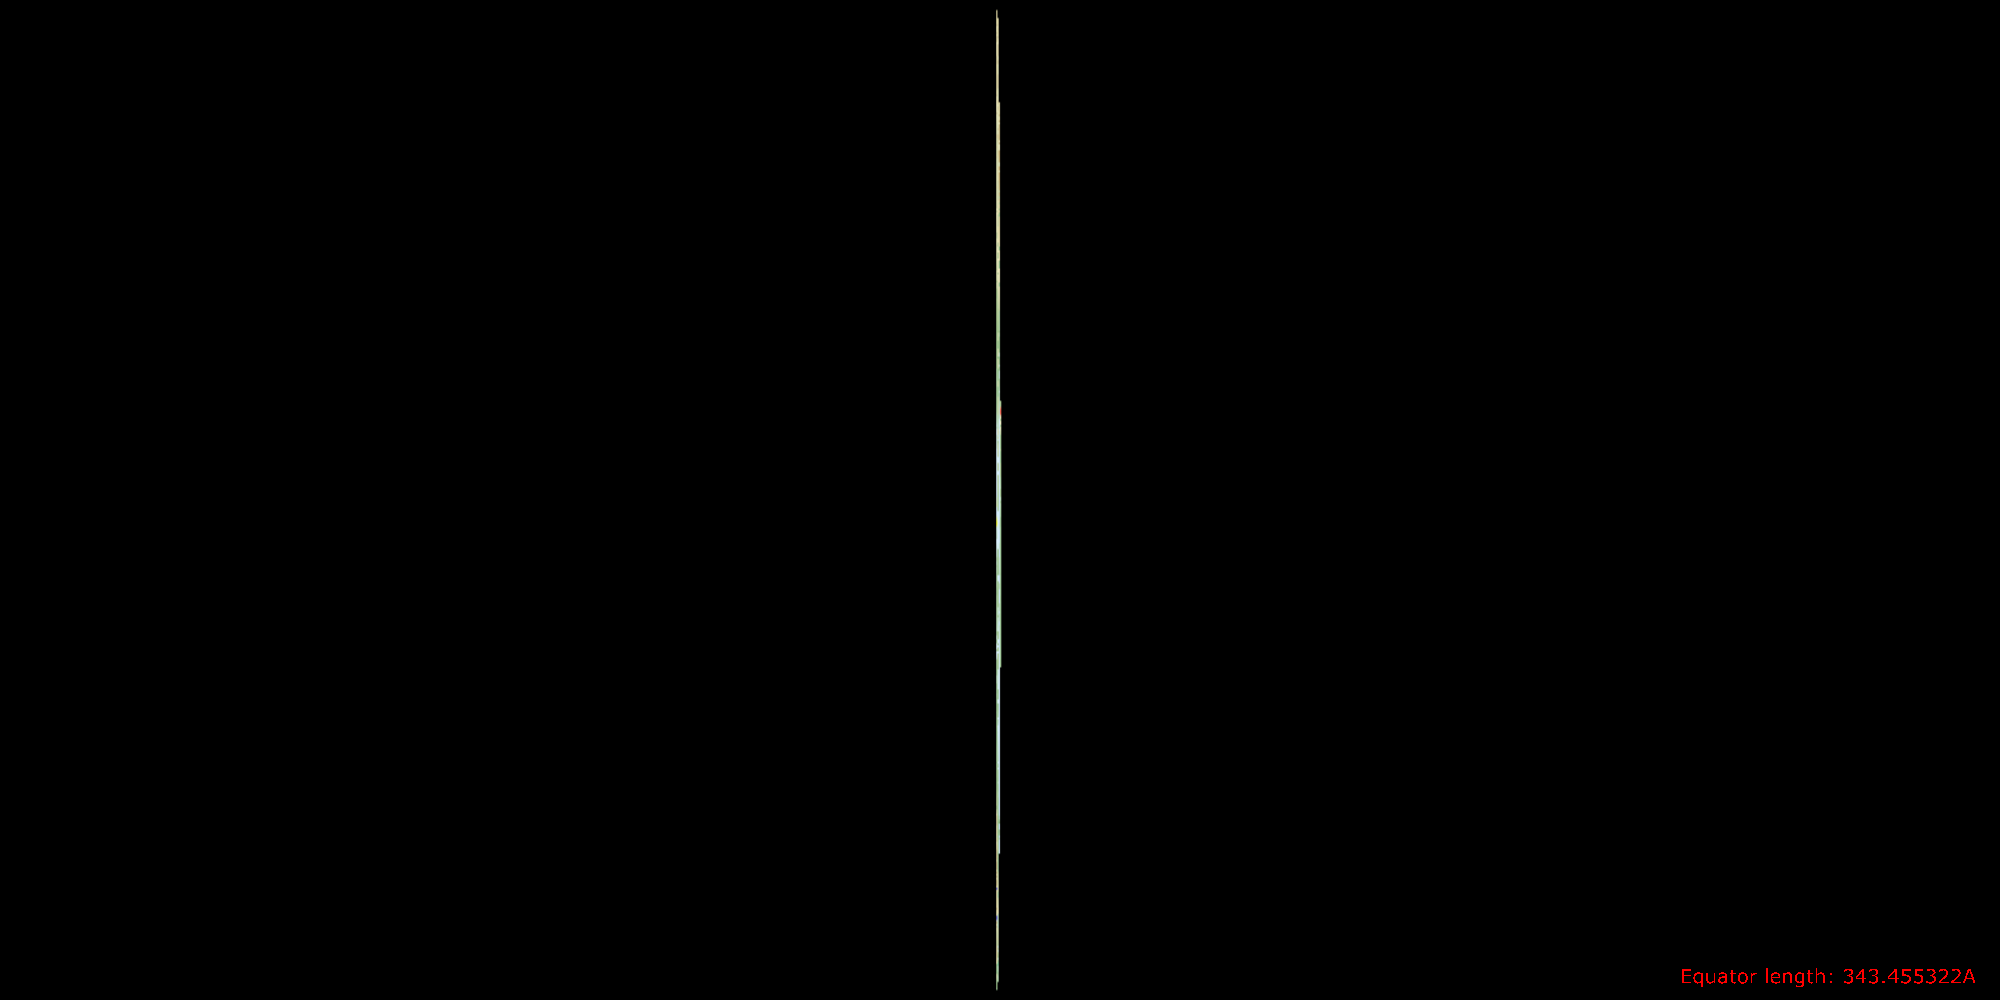
\includegraphics[width=12cm]{teaser}
\caption{Screenshot of a running comvi instance 
}\label{fig:teaser}
}

%%%%%%%%%%%%%%%%%%%%%%%%%%%%%%%%%%%%%%%%%%%%%%%%%%%%%%%%%%%%%%%%
%%%%%%%%%%%%%%%%%%%%%% START OF THE PAPER %%%%%%%%%%%%%%%%%%%%%%
%%%%%%%%%%%%%%%%%%%%%%%%%%%%%%%%%%%%%%%%%%%%%%%%%%%%%%%%%%%%%%%%%

\begin{document}

%% The ``\maketitle'' command must be the first command after the
%% ``\begin{document}'' command. It prepares and prints the title block.

%% the only exception to this rule is the \firstsection command
\firstsection{Introduction}\label{sec:intro}
%
\maketitle
%
\firstsection{Introduction} 
\todo{add sections to tasks in this section}%for journal use above \firstsection{..} instead
Over the span of 6 months we, the authors of this paper,  have researched and implemented a comparative clustering of molecular maps.
The task consisted of several parts: This work was based on the MegaMol project. MegaMol is a simulation tool developed by the Universität Stuttgart and the TU Dresden(?) \todo{cite megamol}\cite{MegaMol}. It can be used to visualize particle data, simulations on atomic scale and other molecular processes. 
Due to its modular nature, it can be extended with modules to interact with other modules.
In this paper we guide you through the \todo{verbose} \verb|MSMCLUSTER| plugin, its capabilities and inner workings.

The next task was to retrieve molecular image data through existing MegaMol plugins \todo{cite moleculr maps}\cite{molecularmaps}. For this a special binary of megamol was compiled and will be released in a separate project \todo{make github link tocomvi public }.
The next task was to extract a expressive feature vector from those images and to find a metric to cluster them by similarity.

The last task which was also developed in a plugin in MagaMol was the visualization on the VISUS POWERWALL. The POWERWALL is a very high definition display that can be used to visualize large data(sets). Due to its size its possible to display much more information than on a regular screen. 

The POWERWALL also supports a tracker device that can transmit 6 degrees of freedom, so for the interaction step we had more freedom to work with than with traditional human interaction devices  \todo{HID abbreviation correct (?)}, for this last step we also researched the possible interactions with the tracking devices on the POWERWALL.

Over the cours of the next few pages you will learn how we approached these challenges and how we (attempted) solved them, what worked and what didn't.

%-------------------------------------------------------------------------
\section{Related Work}\label{sec:relatedWork}

\todo{cite kolesar for clustering}
Clustering proteins by similarity or at least comparing individual proteins has been subject of existing work.

The paper \cite{kolesar} already had similar approaches to our results. Kolesar et al. used a 10 dimensional feature vector based on invariant image moments defined by hu \todo{cite hu image moments} \cite{humoments}

Another approach for 3D protein data were 3D zernicke moments explored by \todo{3d surfer } \cite{3dsurfer}. The approach is basically the same as in Kolesar et al. but the TODO used Zernicke moments instead of traditional image moments and extended them to three dimensions.



\subsection{Initial Challenges and encountered problems}

It is clear that the task required from us that we learn how to compare the images, measure the distances between the images, and cluster these images.
The given task required that we use a similarity based clustering algorithm.

Initially we were given the choice we could either chose to find similarities and cluster the proteins in the \verb|.pdb| format or given as bitmap image generated by the \verb|MolecularMaps| plugin in MegaMol \todo{cite megamol protein image}\cite{molecularmaps}.

Since handling image files which give information about the protein in two dimensions was easier than dealing with the pdb file format which results in three dimensional visualizations we decided to start with a two dimensional approach.





\subsection{Approaches to the Clustering-Problem}

Right of the start we had several ideas of how we could approach this problem. 
With the recent trend in machine learning we had a couple of ideas of how we could determine a similarity metric between two images or classify an image into a more usable vector of data.

We ended up using a higher dimensional feature vector described in \todo{give section label} to determine the similarirty between two protein maps because we didnt manage to train a custom model in the given timeframe, due to inexperience \todo{this can be said better}and non existance of labeled data.

But our relatively spartan results with a pretrained Imagenet \todo{cite imagenet} \cite{imagenet} \todo{cite darknet publication}  model let us to believe that given the knowledge on the subject and humanly labeled data (based on known featuresit \todo{LEFT OFF HERE}shoud be definetly possible for this specified task to find a machine learning  solution using neural networks/autoencoders.

\subsection{Approaches to the Visualization-Task}

Our aproaches to visualizing the given clusters were the following, the reader is reminded that we are not just visualizing the clusters on a ''normal machine'' but rather the POWERWALL, a projected display with effectively 6-24 times the resolution of a consumer grade display. Details on the POWERWALL can be found \todo{cite powerwall publicatoin here if available}. \cite{powerwall}

If we are given so much pixel real estate we are given the freedom to draw smaller pixels since we still will be able to see them on the POWERWALL.

During the duration of the project the idea of a 3D visualization was discussed among the team, but we settled for a 2D visualization. This had a couple of reasons.

While the interactions with the data in 3D would have been more fun since we had more degrees of freedom to work with.
But we could not find a way to present the data in a way such that with just a glance the user could intuitively interpret the data that would be displayed on the screen.

... So we decided to settle for a 2D visualization. Our approach is rather boring but it works. On startup we display nothing, if the user chooses his supplied image data and the algorithms used to cluster the pictures he gets the option to start the visualization.

The visualizatoin consists of displaying the image of a cluster representative with a simple rectangle. 
This way the user knows exactly what to expect to be in the cluster.

If the user wishes to have a closer look at the images in the given cluster he can click onto the representative and will get a view of all the images in that cluster.

We decided after testing with toy test and real datasets that one level of subclustering is enough, after 2 levels of subclustering the clusters get \todo{find better expression}  noisy and ambiguous.

In both the main and subcluster view the representatives are visualized with "force directed layout", to avoid 



\subsubsection{Approaches to the Interaction with the Powerwall \todo{cite correct pub and use correct name}}

\todo{@shoma @enis @damir interaktionsmöglichkeiten schreiben}


\subsection{Finding a feature vector to cluster the images}

The challenge of finding a good feature vector was/is to find good features which are \todo{aussagekräfting} about the image.

The following procedure after finding/determining/calculating the feature vector for a given image is to apply some sort of dimensionality reduction to project a higher dimensional vector onto a 2D or 3D plane.

This has multiuple advantages. First If the dimensionality reduction works as intented one find out after applying the dimensionality reduction if similar looking items are positioned next to each other.

Another reason is the curse of dimensionality. As we all know in higher/infinite dimensional spaces, otherwise unexpected things start to happen such as the euclidian distance or mathimatically put the \begin{equation} L_2 \end{equation}-norm loses relevance since
 \begin{equation}
   \lim_{n\rightarrow \infty} x^n = 0 \quad \forall x \in [0,1)
\end{equation}

Simply put, otherwise very similar values get skewed to zero.

So we have to come up with other solutions to this problem discussed in \todo{put clustering section here}


\todo{back to finding the feature vector}
After looking at a small subset of molecular map images from a variety of proteins we determined that we needed to extract feature information about the follwoing properties of a given image: 

Color distribution, Shape, Texture and image moments 

The initial idea was that the color distribution gives information about the color palette in the image, the extracted shape features should give information about the the biggest \( n \) shapes in the picture, the texture feature should differentiate between smooth and rough texture and everything in between.

The image moments were chosen as a goto approach to extract invariant features from the image which has been proved to yield results as described in \cite{kolesar}

The exact image features that we extract from the image are the following:

\subsection{Invariant Image Moments by Hu}

The set of invariant Image Moments discovered by Hu et. al \todo{find out if hu moments just him or others or et al.} are rotation, translation, scale and trasformation \todo{find out if correct} invariant. This allows us to determine if an image$I_a$ is similar to another image $I_B$ if $I_B$ is equal $I_A$ and simply rotated by $30^°$ \todo{put the value in degrees there}

The (continouus (spelling?)  Image ) Moments  over two dimensions at their core are defined as such:

\[m_{i,j} = \int^\infty_{- \infty}\int^\infty_{- \infty} f(x,y) dy dx \]. When dealing with discrete values like we find them in an (RGB/GS) Image we use sums insteads of integral so we get this:
\[m_{i,j} = \sum^n_{i=0}\sum^m_{j=0} f(i,y) \].\todo{get definition of moment}

Hu further defines his moments as such:
 
\todo{give the definition of all 7/8 moments (?) because this is going to take up a lot of space. }

Kolesar ended up using these moments \todo{put in kolsar moments}, in our case the moments \todo{put the hu moments here}

\subsection{Color palette/histogram }

The goal when extracting color palette was to reduce the big color space that is present in any of the molecular maps and get a few distinct \todo{aussagekräfting} colors from that range.

To achieve this we extract a histogram of each color channel of the RGB images. Each channel is then represented as a greyscale image. We then create for each channel a histogram of the luminance intensities with in our case 16 bins. This "reduces" the \(128*128 = 16384\) dimensions to just \(48\) dimensions for our image.

Alternatively you can take another approach described here

The results of both approaches will be discussed in \todo{cite}

\subsection{Texture}
\todo{better introduction}
After looking at a toy dataset of molecular maps we noticed that many samples had a distinct roughness that looked like they could be used to classify their texture.

We ended up using the haralick textural features. The haralick features work with a grey level correlation matrix (GCM). The gcm for a given greyscale image is defined as such:

\[\text{put the formula here, this is spaceholder}\]

Further value can be take n from this matrix which gives us more features

we also computed this on every channel yielding us another \(x\) features \todo{expand texture features}

\subsection{Shape}

\subsection{Finding the best performing similarity measure}
\subsection{Finding the best performing clustering algorithm}
\subsection{Testing the feature vector with other datasets}
\begin{figure}
  \begin{center}
  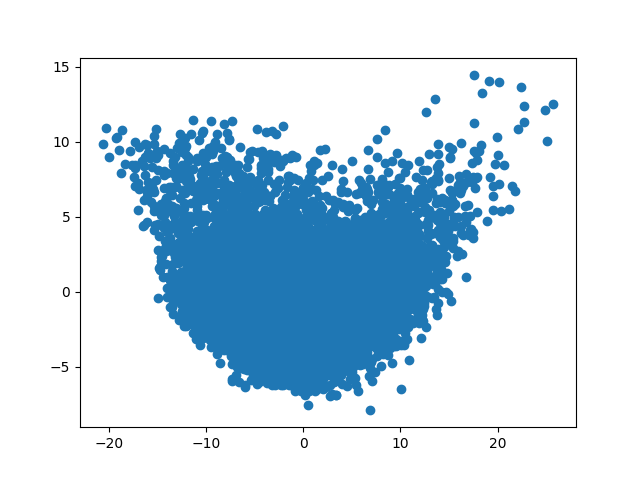
\includegraphics[width=.6\linewidth]{Figure1.png}
  \end{center}
  \caption{\label{fig:lorem} Early test with the Oxford flower dataset \todo{cite oxford flower dataset}}
\end{figure} ~ \\
\begin{figure}
  \begin{center}
  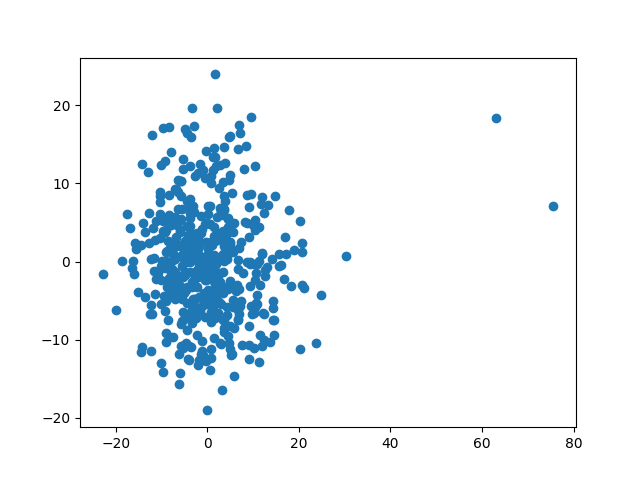
\includegraphics[width=.6\linewidth]{Figure2.png}
  \end{center}
  \caption{\label{fig:bmw} Early test with the bmw car dataset \todo{cite stanford car dataset}\cite{stanfordcar}}
\end{figure}
\subsection{Finding the }
\subsection{Discussion of results}
\subsubsection{Dolor}

\begin{table}
\caption{
\label{tab:perf} lorem ipsum tabulated}
\centering
\vspace{0.3em}
\begin{tabular}{lrr}
dataset & full performance (fps) & half performance (ms)\\ \hline\\[-0.4em]
balls & 1,243 & 0.1 \\
buckets & 23 & 23 \\
bolts & 23,312,134.3 & 22.1 \\
\end{tabular}
\end{table}



%% if specified like this the section will be ommitted in review mode
\acknowledgments{
We would like to thank our supervisors Michael Krone and Florian Fries as well as our project examiner Prof. Ertl, for giving us this opportunity to work on this project. We are grateful that we were able to improve and learn. We are also grateful for the feedback we recieved on our work. \\
This work was partially funded by cake and cookies.
}

\bibliographystyle{abbrv}
%%use following if all content of bibtex file should be shown
%\nocite{*}
\bibliography{template}
\end{document} 
